\section{Results}
In this section, I will present the performance of both the machine learning and deep learning models on the sarcasm detection task. The evaluation metrics include accuracy, F1 score, 
recall, and precision. In addition, confusion matrices provide further insight into each model's performance by detailing the distribution of true positives, true negatives, 
false positives, and false negatives.

\subsection{Machine Learning Models Results}

Table \ref{Table_1} summarizes the performance metrics for the four machine learning models that were tested using both TF-IDF and Bag-of-Words (BoW) representations.

\begin{table}
    \caption{Machine Learning Models Results}
    \label{Table_1}
    \begin{tabular}{ccccc}
        \toprule
            \textbf{Model} & \textbf{Accuracy (\%)} & \textbf{F1 Score (\%)} & \textbf{Recall (\%)} & \textbf{Precision (\%)} \\
        \midrule
            Logistic Regression (TF-IDF)  & 71.9 & 70.7 & 67.7 & 73.9 \\
            Ridge Regression (TF-IDF)     & 71.5 & 70.5 & 68.2 & 73.0 \\
            Logistic Regression (BoW)     & 71.9 & 70.4 & 66.9 & 74.3 \\
            Ridge Regression (BoW)        & 71.2 & 69.5 & 65.7 & 73.8 \\
         \bottomrule
    \end{tabular}
\end{table}

Logistic Regression model with TF-IDF achieved an accuracy of 71.9\% and an F1 score of 70.7\%. The confusion matrix reveals 273,531 true positives and 307,988 true negatives, 
with 96,334 false positives and 130,741 false negatives. While the model demonstrates a reasonably strong performance overall, the relatively high number of false negatives suggests that it sometimes 
fails to detect sarcasm, misclassifying sarcastic comments as normal.

Ridge Regression with TF-IDF achieved slightly lower accuracy at 71.5\% and an F1 score of 70.5\%. This model recorded 275,560 true positives and 302,802 true negatives, 
with 101,520 false positives and 128,712 false negatives. Compared to Logistic Regression (TF-IDF), it is marginally more aggressive in predicting sarcasm, as indicated by the higher 
false positive count, although it does slightly better in terms of capturing sarcastic instances (fewer false negatives).

When using a BoW representation, Logistic Regression obtained an accuracy of 71.9\% and an F1 score of 70.4\%. The confusion matrix shows 270,556 true positives and 310,948 true negatives, 
with 93,374 false positives and 133,716 false negatives. This model correctly classifies a higher number of normal comments, as indicated by the increased true negative count and reduced 
false positives. However, this comes at the cost of a higher number of false negatives, meaning that it misses a greater number of sarcastic comments.

Ridge Regression with BoW achieved an accuracy of 71.2\% and an F1 score of 69.5\%. Its confusion matrix reveals 265,506 true positives and 310,275 true negatives, along with 
94,047 false positives and the highest number of false negatives at 138,766. This model struggles most with detecting sarcastic comments, as evidenced by its high false negative count, 
even though it performs well in correctly identifying normal comments.

Overall, TF-IDF-based models provide a better balance between false positives and false negatives compared to their BoW counterparts. Among these, Logistic Regression with TF-IDF offers 
the best trade-off, achieving high accuracy while minimizing misclassifications. This model was trained on the full dataset and obtained an accuracy of 72.23\%. The confusion matrices 
for the models are available in Figure \ref{Fig_4}.

\begin{figure}
    \centering
    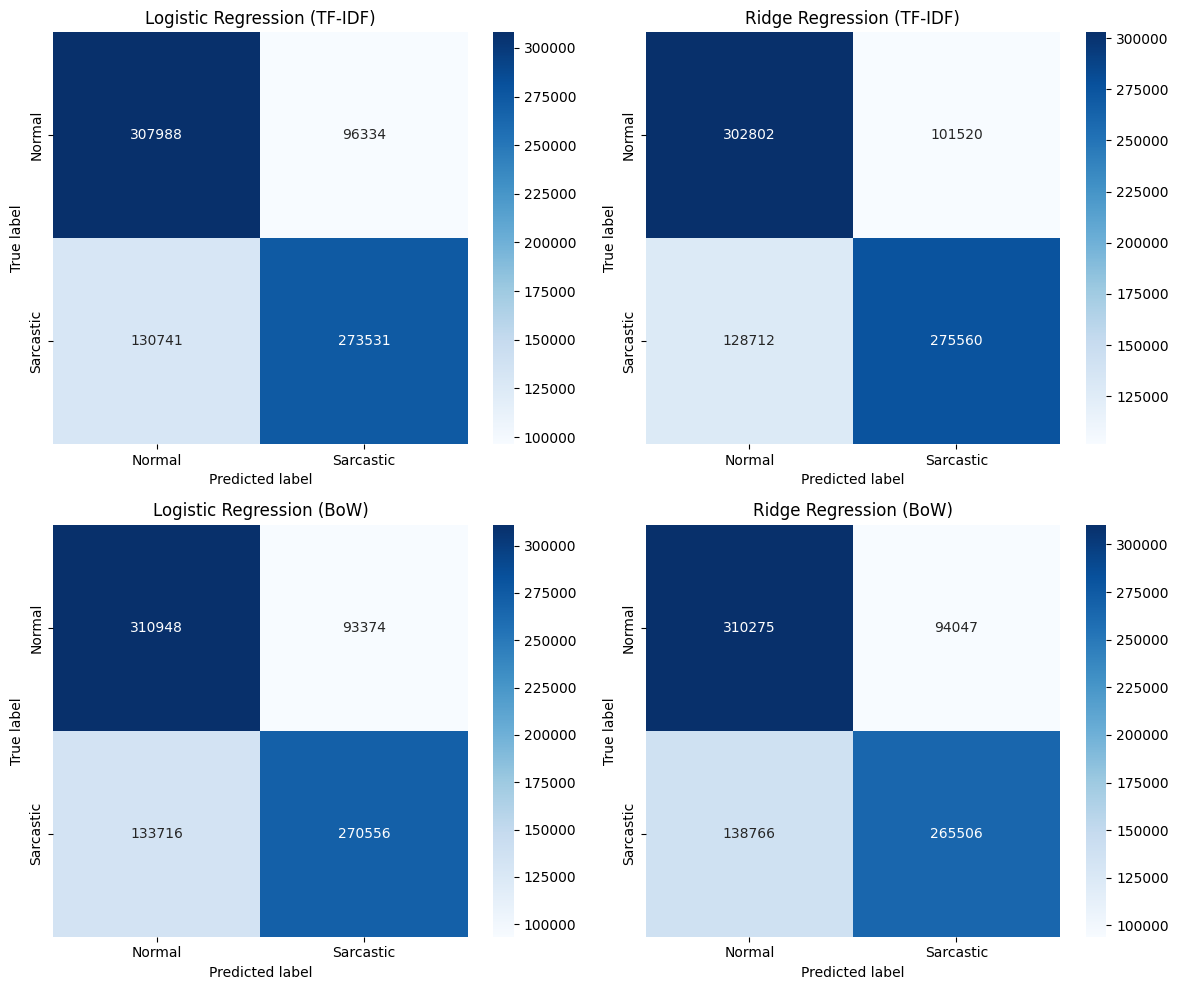
\includegraphics[width=0.8\linewidth]{img/conf_matrix.png}
    \caption{Confusion Matrices}
    \label{Fig_4}
\end{figure}
